\documentclass[dvipdfmx]{jsarticle}
\usepackage{tikz}
\usepackage{amsmath}
\usepackage{url}
\newcommand{\cat}[1]{\boldsymbol{#1}}
\newcommand{\catcat}{\mathbf{Cat}}
\newcommand{\arrow}{\rightarrow}
\newcommand{\functor}[3]{#1:\cat{#2}\arrow \cat{#3}}
\newcommand{\nat}{\Rightarrow}
\newcommand{\tuple}[1]{\langle #1\rangle}
\newcommand{\obj}[1]{Obj(\cat{#1})}
\newcommand{\mor}[3]{#1:#2\arrow #3}

\newtheorem{proof}{証明}[section]
\newtheorem{prop}{命題}[section]
\newtheorem{define}{定義}[section]
\numberwithin{proof}{subsection}
\numberwithin{prop}{subsection}
\numberwithin{define}{subsection}
\begin{document}
	\title{圏論入門}
	\maketitle
	\tableofcontents
	\section{はじめに}
	圏論は抽象代数学で生まれ、現在では代数学、幾何学、数学基礎論や、計算機科学、言語学、認知科学、哲学などにも応用されている。
	本資料は数学基礎論や計算機科学で特に使われるデカルト閉圏を中心に解説していく。
	また他の入門書の差別化として、できるだけ議論や具体例を圏論の中で完結するようにしている。
	\section{圏と公理}

	\begin{define}
		ある圏$\cat{C}$は、以下の要素と演算、公理から構成される。
		\begin{description}
			\item[対象] 対象の集合$\obj{C}\ni A,B,C...$
			\item[射] 射の集合$Mor(\cat{C})\ni f,g,h...$
			\item[ドメインとコドメイン]~\\ 射から対象への二つの演算$dom,cod$、もし$dom(f)=A$、$cod(f)=B$であれば、$f\in Mor(A,B)$または$\mor{f}{A}{B}$と表す。
			また、$f$に対する$dom(f)$をドメイン、$cod(f)$をコドメインと呼ぶ。

			ある対象$A,B,C$、ある射$\mor{f}{A}{B}$、$\mor{g}{A}{C}$、$\mor{h}{C}{B}$について考えるとき、以下のような図式を用いて議論を行うことがある。
			\begin{center}
				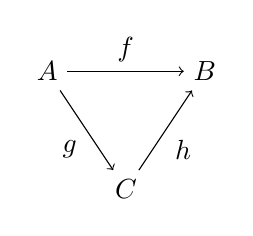
\begin{tikzpicture}[auto]
					\node (a) at (0, 0) {$A$};
					\node (b) at (2, 0) {$B$};
					\node (c) at (1, -1.5) {$C$};
					\draw[->] (a) to node {$f$}(b);
					\draw[->] (a) to node[swap] {$g$}(c);
					\draw[->] (c) to node[swap] {$h$}(b);
				\end{tikzpicture}
			\end{center}

			\item[射の合成]~\\ ある射$f,g$が$cod(f)=dom(g)$を満たす、つまり$\mor{f}{X}{A}$、$\mor{g}{A}{Y}$であるようなとき、射の合成$\mor{g\circ f}{X}{Y}$が行える。
			射をつなげる、という直感に反して合成射の射の順序が射の向きと逆であることに注意してほしい。

			射$h,g$の合成$h\circ g$は次のように表せる。
			また対象$A$と対象$B$の間の射は一つとは限らないので、必ずしも$h\circ g=f$が成り立つわけではない。
			\begin{center}
				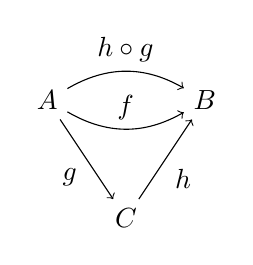
\begin{tikzpicture}[auto]
					\node (a) at (0, 0) {$A$};
					\node (b) at (2, 0) {$B$};
					\node (c) at (1, -1.5) {$C$};
					\draw[->] (a) to[bend right=30] node {$f$}(b);
					\draw[->] (a) to[bend right=-30] node {$h\circ g$}(b);
					\draw[->] (a) to node[swap] {$g$}(c);
					\draw[->] (c) to node[swap] {$h$}(b);
				\end{tikzpicture}
			\end{center}
			\item[恒等射の存在] 恒等射と呼ばれる特別な射$\mor{id_A}{A}{A}$が任意の対象に存在する。
			\item[結合律] 結合則$h\circ (g\circ f)=(h\circ g)\circ f$が合成可能な任意の射$f,g,h$で成り立つ。

				\begin{center}
				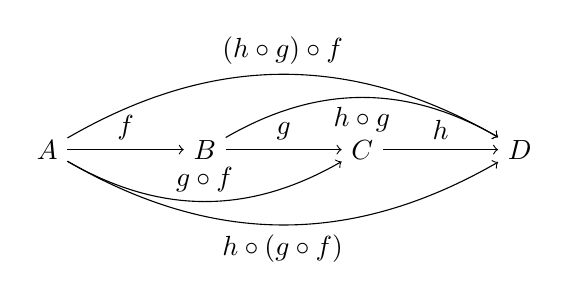
\begin{tikzpicture}[auto]
					\node (a) at (0, 0) {$A$};
					\node (b) at (2, 0) {$B$};
					\node (c) at (4, 0) {$C$};
					\node (d) at (6, 0) {$D$};
					\draw[->] (a) to node {$f$}(b);
					\draw[->] (b) to node {$g$}(c);
					\draw[->] (c) to node {$h$}(d);
					\draw[->] (a) to[bend right=30] node {$g\circ f$}(c);
					\draw[->] (a) to[bend right=30] node[swap] {$h\circ(g\circ f)$}(d);
					\draw[->] (b) to[bend left=30] node[swap] {$h\circ g$}(d);
					\draw[->] (a) to[bend left=30] node {$(h\circ g)\circ f$}(d);
				\end{tikzpicture}
			\end{center}
			\item[単位元律]~\\ 任意の対象$A$と対応する恒等射$\mor{id_A}{A}{A}$、任意の射$\mor{f}{X}{A}$、$\mor{g}{A}{Y}$において$id_A\circ f=f$、$g\circ id_A=g$が成り立つ。

			恒等射をある射に合成しても、合成する前の射と等しくなることから、直感的に恒等射は何も行わない射のように考えられる。

			\begin{center}
				\begin{tikzpicture}[auto]
					\node (x) at (0, 0) {$X$};
					\node (a) at (2, 0) {$A$};
					\node (y) at (4, 0) {$Y$};
					\draw[->] (x) to node {$f$}(a);
					\draw[->,loop above, looseness=20] (a) to node {$id_A$}(a);
					\draw[->] (a) to node {$g$}(y);
				\end{tikzpicture}
				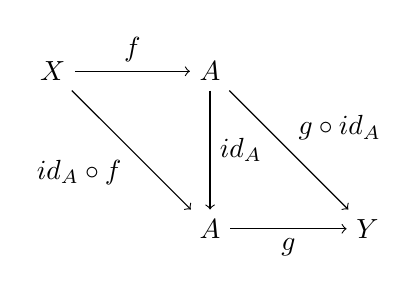
\begin{tikzpicture}[auto]
					\node (a) at (0, 0) {$X$};
					\node (b) at (2, 0) {$A$};
					\node (b') at (2, -2) {$A$};
					\node (c) at (4, -2) {$Y$};
					\draw[->] (a) to node {$f$}(b);
					\draw[->] (b) to node {$id_A$}(b');
					\draw[->] (b') to node[swap]  {$g$}(c);
					\draw[->] (a) to node[swap]  {$id_A\circ f$}(b');
					\draw[->] (b) to node {$g\circ id_A$}(c);
				\end{tikzpicture}
			\end{center}
		\end{description}
	\end{define}
	\section{圏論の基本概念}
	圏論では対象の性質をその対象をドメイン、コドメインとする射の性質によって与える。
	直感的にはある対象を述べる場合、「どのように構成されるか」ではなく「どのように振舞うか」で述べるように思える。

	まずはこれまで図示してきた図式について数学的な定義を与える。
	\begin{define}[図式(部分圏)]
		ある圏$\cat{C}$のある図式(部分圏)とは、圏$\cat{C}$に含まれるいくつかの対象と、いくつかの射で構成される圏であり、任意の対象に対応する恒等射を含み、図式中の任意の合成可能な二射$\mor{f}{X}{Y},\mor{g}{Y}{Z}$が含まれるとき、その合成射$g\circ f$も含むような圏である。
	\end{define}
	また図式は単に図示するために使用する以外にも、圏論のいくつかの概念を定義するのにも用いられる。
	\begin{define}[可換]
		圏におけるいくつかの射と対象の集まりである図式が可換である。すなわち可換図式であるとは、図式中の対象を頂点、図式中の射を辺とする有向グラフを考えたとき、任意の頂点$C,C'$において$C$から$C'$への任意の経路によって表される射が等しいときである。
	\end{define}
	例えば以下の図式において$j\circ g=l\circ i,k\circ h=m\circ j,k\circ h\circ g=m\circ j\circ g = m\circ l\circ i$が成り立つとすると、これは可換図式になる。

	\begin{center}
		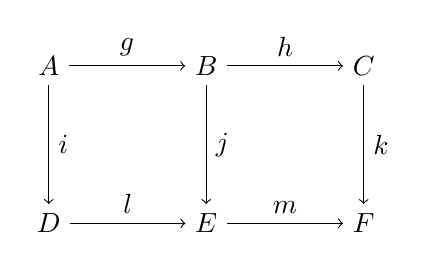
\begin{tikzpicture}[auto]
			\node (a) at (0, 0) {$A$};
			\node (b) at (2, 0) {$B$};
			\node (c) at (4, 0) {$C$};
			\node (d) at (0, -2) {$D$};
			\node (e) at (2, -2) {$E$};
			\node (f) at (4, -2) {$F$};
			\draw[->] (a) to node {$g$}(b);
			\draw[->] (b) to node {$h$}(c);
			\draw[->] (a) to node {$i$}(d);
			\draw[->] (b) to node {$j$}(e);
			\draw[->] (c) to node {$k$}(f);
			\draw[->] (d) to node {$l$}(e);
			\draw[->] (e) to node {$m$}(f);
		\end{tikzpicture}
	\end{center}

	\subsection{元}
		集合論では集合から集合への関数の性質を述べるのに集合の元を用いることが多いが、圏の対象では一般的に元を取ることができない。
		しかしある圏$\cat{C}$に終対象$1$と呼ばれる特別な対象が存在するとき、$\cat{C}$の任意の対象$A$のある元(global elements)はある射$\mor{a}{1}{A}$で表せる。
		\begin{center}
			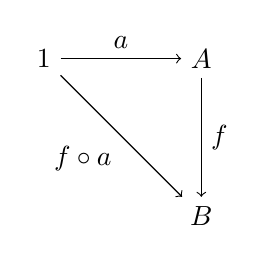
\begin{tikzpicture}[auto]
				\node (a) at (2, 0) {$A$};
				\node (b) at (2, -2) {$B$};
				\node (1) at (0, 0) {$1$};
				\draw[->] (1) to node {$a$}(a);
				\draw[->] (1) to node[swap] {$f\circ a$}(b);
				\draw[->] (a) to node {$f$}(b);
			\end{tikzpicture}
		\end{center}

		射$\mor{f}{A}{B}$に対して$\mor{a}{1}{A}$を適用する操作は、そのまま関数の合成$\mor{f\circ a}{1}{B}$で表せる。
		また射を適用した元もまた終対象からの射になるから$f\circ a$もまた対象$B$の元になる。
		終対象の定義や、ある対象と終対象からその対象への射の全体が等価になることについては、当分先になるであろうが後に説明する。
		任意の圏に終対象が存在するわけではないが、これから説明する圏論の概念たちの解説に使用するためここで軽く説明した。
	\subsection{同型}
	圏論では対象の性質を射の性質で説明すると述べたが、対象の等しさを射の等しさで説明した同型という概念がある。
	\begin{define}[同型]
		ある対象$A$と$B$が同型、つまり$A\cong B$であるとは、$f\circ f^{-1}=id_B$と$f^{-1}\circ f=id_A$を満たすようなある二つの射$\mor{f}{A}{B}$とその逆射$\mor{f^{-1}}{B}{A}$が存在するときである。
		また、このような射$f,f^{-1}$を同型射と呼ぶ。
	\end{define}
	\begin{center}
		\begin{tikzpicture}[auto]
			\node (a) at (-4, -1) {$A$};
			\node (b) at (-2, -1) {$B$};
			\draw[->,transform canvas={yshift=-3pt}] (a) to node[swap] {$f$}(b);
			\draw[->,transform canvas={yshift=3pt}] (b) to node[swap] {$f^{-1}$}(a);

			\node (a) at (0, 0) {$A$};
			\node (b) at (2, 0) {$B$};
			\node (b') at (0, -2) {$B$};
			\draw[->] (a) to node[swap] {$f$}(b');
			\draw[->] (b) to node {$id_B$}(b');
			\draw[->] (b) to node[swap] {$f^{-1}$}(a);

			\node (a) at (4, 0) {$B$};
			\node (b) at (6, 0) {$A$};
			\node (b') at (4, -2) {$A$};
			\draw[->] (a) to node[swap] {$f^{-1}$}(b');
			\draw[->] (b) to node {$id_A$}(b');
			\draw[->] (b) to node[swap] {$f$}(a);
		\end{tikzpicture}
	\end{center}
	\subsection{演習問題}
	\begin{enumerate}
		\item 以下の図式において左側の正方形の図式と右側の正方形の図式がそれぞれ可換になるとき、二つを合わせた長方形の図式が可換になることを示せ。
			\begin{center}
				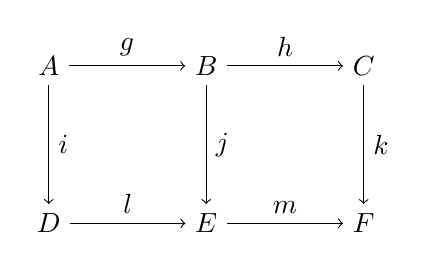
\begin{tikzpicture}[auto]
					\node (a) at (0, 0) {$A$};
					\node (b) at (2, 0) {$B$};
					\node (c) at (4, 0) {$C$};
					\node (d) at (0, -2) {$D$};
					\node (e) at (2, -2) {$E$};
					\node (f) at (4, -2) {$F$};
					\draw[->] (a) to node {$g$}(b);
					\draw[->] (b) to node {$h$}(c);
					\draw[->] (a) to node {$i$}(d);
					\draw[->] (b) to node {$j$}(e);
					\draw[->] (c) to node {$k$}(f);
					\draw[->] (d) to node {$l$}(e);
					\draw[->] (e) to node {$m$}(f);
				\end{tikzpicture}
				\begin{tikzpicture}[auto]
					\node (a) at (4, 0) {$A$};
					\node (c) at (8, 0) {$C$};
					\node (d) at (4, -2) {$D$};
					\node (f) at (8, -2) {$F$};
					\draw[->] (a) to node {$h\circ g$}(c);
					\draw[->] (d) to node {$m\circ l$}(f);
					\draw[->] (a) to node {$i$}(d);
					\draw[->] (c) to node {$k$}(f);
				\end{tikzpicture}
			\end{center}
		\item $A\cong B$かつ$B\cong C$ならば$A\cong C$であることを示せ。
	\end{enumerate}

	\section{普遍性}
	普遍性はある対象と射を特徴づけるために使用され、ある図式を可換にするような射が一意に定まる。というように記述され、図式中の射と一意に定まる射の対応関係を示すことが多い。
	\subsection{積}
	\begin{define}[積]
		対象$A$と$B$が積を持つとは、以下の条件を満たす組$(A\times B,\pi_A,\pi_B)$が存在するときである。
		\begin{description}
		\item[積対象と射影射]ある積対象$A\times B$とある二つの射$\mor{\pi_A}{A\times B}{A}$、$\mor{\pi_B}{A\times B}{B}$が存在する。
		この時、積対象と射影射の組$(A\times B,\pi_A,\pi_B)$を$A,B$の積と呼ぶ。
		\item[任意の対象からの射]任意の対象$X$と二つの射$\mor{f}{X}{A}$、$\mor{g}{X}{B}$の組を$(X,f,g)$とする。
		\item[射の対]任意の組$(X,f,g)$に対して射の対と呼ばれる射$\mor{\tuple{f,g}}{X}{A\times B}$が存在する。
		\item[普遍性]射の対は図式を可換にし、$(X,f,g)$に対して一意に定まる。
		すなわち、$\pi_A\circ\tuple{f,g}=f$、$\pi_B\circ\tuple{f,g}=g$が成り立つような$\tuple{f,g}$が一意に定まる。
		\end{description}
		\begin{center}
			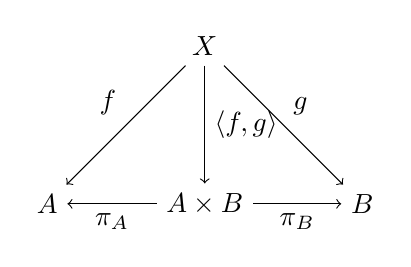
\begin{tikzpicture}[auto]
				\node (a) at (0, 0) {$A$};
				\node (b) at (4, 0) {$B$};
				\node (ab) at (2, 0) {$A\times B$};
				\node (x) at (2, 2) {$X$};
				\draw[->] (ab) to node {$\pi_A$}(a);
				\draw[->] (ab) to node[swap] {$\pi_B$}(b);
				\draw[->] (x) to node[swap] {$f$}(a);
				\draw[->] (x) to node {$g$}(b);
				\draw[->] (x) to node {$\tuple{f,g}$}(ab);
			\end{tikzpicture}
		\end{center}
		すべての圏、すべての二対象に対して積が存在するとは限らないが、ある圏$\cat{C}$の任意の二対象に対して積が存在するとき、圏$\cat{C}$は積を持つという。
	\end{define}

	つまり、ある射$\mor{h}{X}{A\times B}$が存在して$\pi_A\circ h=f$、$\pi_B\circ h=g$を満たすとき、このような射は一意に存在するから$h=\tuple{f,g}$となる。

	ここで$X$に終対象$1$を当てはめると、$A$のある元$a$、$B$のある元$b$に対して$\pi_A\circ\tuple{a,b}=a$、$\pi_B\circ\tuple{a,b}=b$が成り立つような$\tuple{a,b}$が一意に定まる。
	直感的には$\pi_A$と$\pi_B$は$A\times B$の元$\tuple{a,b}$からそれぞれ$A$の元と$B$の元を取りだす。もし$A\times B$のまた別の元$\mor{h}{1}{A\times B}$からも$a$と$b$が取り出せたなら、$h=\tuple{a,b}$となることがわかる。

	\begin{center}
		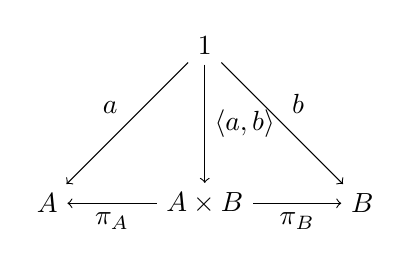
\begin{tikzpicture}[auto]
			\node (a) at (0, 0) {$A$};
			\node (b) at (4, 0) {$B$};
			\node (ab) at (2, 0) {$A\times B$};
			\node (x) at (2, 2) {$1$};
			\draw[->] (ab) to node {$\pi_A$}(a);
			\draw[->] (ab) to node[swap] {$\pi_B$}(b);
			\draw[->] (x) to node[swap] {$a$}(a);
			\draw[->] (x) to node {$b$}(b);
			\draw[->] (x) to node {$\tuple{a,b}$}(ab);
		\end{tikzpicture}
	\end{center}

	次に積の性質をいくつか見ていく。
	\begin{prop}[射の対の分配則]
		$\mor{f}{X}{A}$、$\mor{g}{X}{B}$、$\mor{h}{Y}{X}$に対して$\tuple{f,g}\circ h=\tuple{f\circ h,g\circ h}$が成り立つ
	\end{prop}
	\begin{proof}
		積$A\times B$に対し、対$(X,f,g)$に$(Y,f\circ h, g\circ h)$を当てはめると、積の普遍性よりこの図式を可換にする射の対$\mor{\tuple{f\circ h,g\circ h}}{Y}{A\times B}$が存在し一意に定まる。
		よって$\tuple{f,g}\circ h=\tuple{f\circ h,g\circ h}$が成り立つ。
	\end{proof}

	\begin{center}
		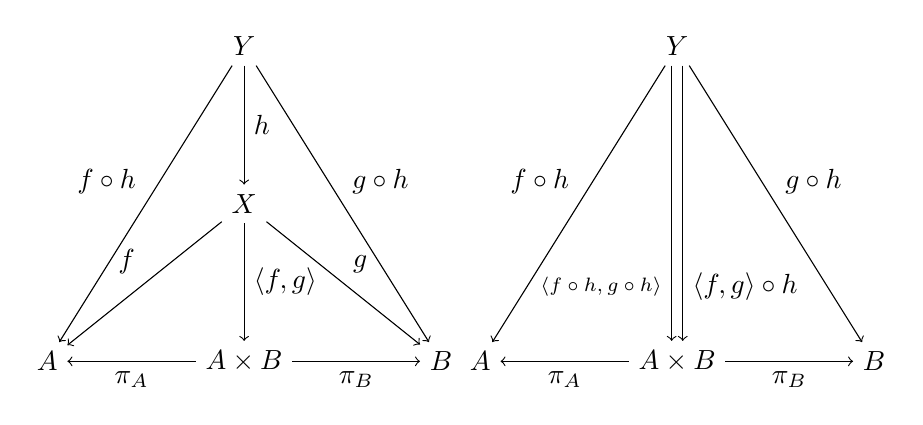
\begin{tikzpicture}[auto]
			\node (y) at (3, 4) {$Y$};
			\node (a) at (0.5, 0) {$A$};
			\node (b) at (5.5, 0) {$B$};
			\node (ab) at (3, 0) {$A\times B$};
			\node (x) at (3, 2) {$X$};
			\draw[->] (y) to node {$h$}(x);
			\draw[->] (y) to node[swap] {$f\circ h$}(a);
			\draw[->] (y) to node {$g\circ h$}(b);
			\draw[->] (ab) to node {$\pi_A$}(a);
			\draw[->] (ab) to node[swap] {$\pi_B$}(b);
			\draw[->] (x) to node[swap] {$f$}(a);
			\draw[->] (x) to node {$g$}(b);
			\draw[->] (x) to node {$\tuple{f,g}$}(ab);

			\node (y) at (8.5, 4) {$Y$};
			\node (a) at (6, 0) {$A$};
			\node (b) at (11, 0) {$B$};
			\node (ab) at (8.5, 0) {$A\times B$};
			\draw[->, transform canvas={xshift=2pt}] (y) to node[yshift=-30pt] {$\tuple{f,g}\circ h$}(ab);
			\draw[->, transform canvas={xshift=-2pt}] (y) to node[yshift=-30pt, swap] {\scriptsize{$\tuple{f\circ h,g\circ h}$}}(ab);
			\draw[->] (y) to node[swap] {$f\circ h$}(a);
			\draw[->] (y) to node {$g\circ h$}(b);
			\draw[->] (ab) to node {$\pi_A$}(a);
			\draw[->] (ab) to node[swap] {$\pi_B$}(b);
		\end{tikzpicture}
	\end{center}
	また$Y$に終対象$1$、$h$に元$\mor{x}{1}{X}$を当てはめると、同様に$\tuple{f,g}\circ x=\tuple{f\circ x,g\circ x}$となる。
	つまり射の対は与えられた元にそれぞれの射を適用し、また対をとするような射だと考えられる。
	\begin{center}
		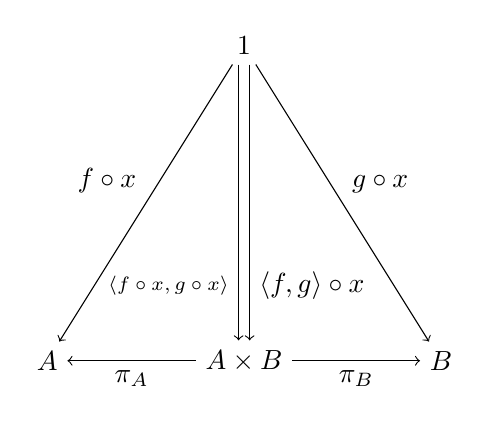
\begin{tikzpicture}[auto]
			\node (y) at (8.5, 4) {$1$};
			\node (a) at (6, 0) {$A$};
			\node (b) at (11, 0) {$B$};
			\node (ab) at (8.5, 0) {$A\times B$};
			\draw[->, transform canvas={xshift=2pt}] (y) to node[yshift=-30pt] {$\tuple{f,g}\circ x$}(ab);
			\draw[->, transform canvas={xshift=-2pt}] (y) to node[yshift=-30pt, swap] {\scriptsize{$\tuple{f\circ x,g\circ x}$}}(ab);
			\draw[->] (y) to node[swap] {$f\circ x$}(a);
			\draw[->] (y) to node {$g\circ x$}(b);
			\draw[->] (ab) to node {$\pi_A$}(a);
			\draw[->] (ab) to node[swap] {$\pi_B$}(b);
		\end{tikzpicture}
	\end{center}

	次に、任意の積から任意の積への射である、射の積を定義していく。
	\begin{define}[射の積]
		射$\mor{f}{A}{A'}$、$\mor{g}{B}{B'}$に対して射の積$\mor{f\times g}{A\times B}{A'\times B'}$を$f\times g = \tuple{f\circ\pi_A,g\circ\pi_B}$と定義する。
		\begin{center}
			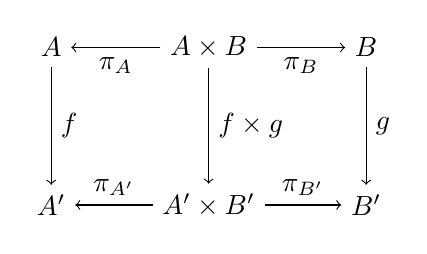
\begin{tikzpicture}[auto]
				\node (a) at (0, 0) {$A$};
				\node (ab) at (2, 0) {$A\times B$};
				\node (b) at (4, 0) {$B$};
				\node (a') at (0, -2) {$A'$};
				\node (a'b') at (2, -2) {$A'\times B'$};
				\node (b') at (4, -2) {$B'$};
				\draw[->] (a'b') to node[swap] {$\pi_{A'}$}(a');
				\draw[->] (a'b') to node {$\pi_{B'}$}(b');
				\draw[->] (ab) to node {$\pi_A$}(a);
				\draw[->] (ab) to node[swap] {$\pi_B$}(b);
				\draw[->] (a) to node {$f$}(a');
				\draw[->] (b) to node {$g$}(b');
				\draw[->] (ab) to node {$f\times g$}(a'b');
			\end{tikzpicture}
		\end{center}
	\end{define}
	射の対は任意の対象から任意の積への射であるのに対し、射の積は任意の積から任意の積への射である。
	二つの対象から二つの対象へ射を一つの射に纏めることから、直感的に射の積は並列処理のように思える。

	\begin{prop}[積と合成の交換]
		射の積$\mor{f\times g}{A\times B}{A'\times B'}$、$\mor{f'\times g'}{A'\times B'}{A''\times B''}$に対して、$(f'\times g')\circ(f\times g)=(f'\circ f)\times(g'\circ g)$が成り立つ。
	\end{prop}
	\begin{proof}
		上の図式と下の図式はそれぞれ射の積の図式であり可換であるため、図式全体も可換になる。

		また積$A''\times B''$において、対$(X,f,g)$に$(A\times B,f'\circ f\circ\pi_A$,$g'\circ g\circ\pi_B)$を当てはめると射$\mor{\tuple{f'\circ f\circ\pi_A,g'\circ g\circ\pi_B}}{A\times B}{A''\times B''}$が存在する。

		また射の積の定義より、$\tuple{f'\circ f\circ\pi_A,g'\circ g\circ\pi_B}=(f'\circ f)\times(g'\circ g)$が成り立つ。

		ここで図式全体が可換になるため、$(f'\times g')\circ(f\times g)$も同様に積の図式を可換にする。よって、射の一意性より、$(f'\times g')\circ(f\times g)=(f'\circ f)\times(g'\circ g)$が成り立つ。
		\begin{center}
			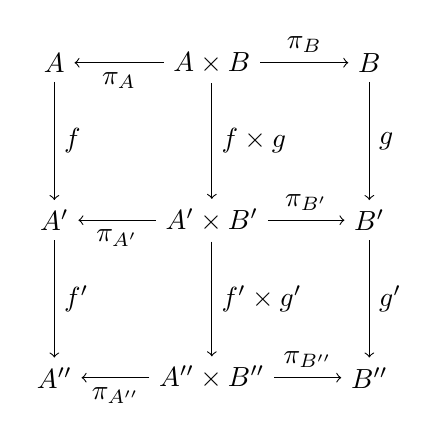
\begin{tikzpicture}[auto]
				\node (a) at (0, 0) {$A$};
				\node (a') at (0, -2) {$A'$};
				\node (a'') at (0, -4) {$A''$};
				\node (ab) at (2, 0) {$A\times B$};
				\node (ab') at (2, -2) {$A'\times B'$};
				\node (ab'') at (2, -4) {$A''\times B''$};
				\node (b) at (4, 0) {$B$};
				\node (b') at (4, -2) {$B'$};
				\node (b'') at (4, -4) {$B''$};
				\draw[->] (ab) to node{$\pi_{A}$}(a);
				\draw[->] (ab) to node{$\pi_{B}$}(b);
				\draw[->] (ab') to node{$\pi_{A'}$}(a');
				\draw[->] (ab') to node{$\pi_{B'}$}(b');
				\draw[->] (ab'') to node{$\pi_{A''}$}(a'');
				\draw[->] (ab'') to node{$\pi_{B''}$}(b'');
				\draw[->] (a) to node{$f$}(a');
				\draw[->] (a') to node{$f'$}(a'');
				\draw[->] (b) to node{$g$}(b');
				\draw[->] (b') to node{$g'$}(b'');
				\draw[->] (ab) to node{$f\times g$}(ab');
				\draw[->] (ab') to node{$f'\times g'$}(ab'');
			\end{tikzpicture}
			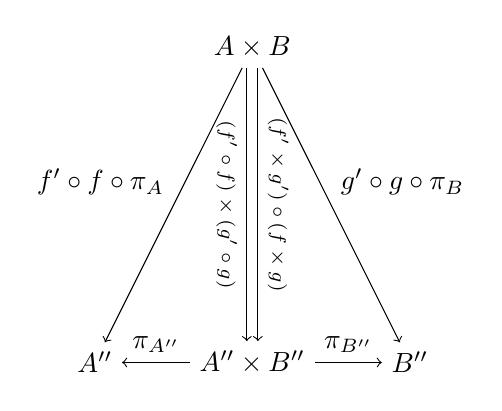
\begin{tikzpicture}[auto]
				\node (a'') at (0, -4) {$A''$};
				\node (ab) at (2, 0) {$A\times B$};
				\node (ab'') at (2, -4) {$A''\times B''$};
				\node (b'') at (4, -4) {$B''$};
				\draw[->] (ab) to node[swap]{$f'\circ f\circ\pi_A$}(a'');
				\draw[->] (ab) to node{$g'\circ g\circ\pi_B$}(b'');
				\draw[->] (ab'') to node[swap]{$\pi_{A''}$}(a'');
				\draw[->] (ab'') to node{$\pi_{B''}$}(b'');
				\draw[->,transform canvas={xshift=2pt}] (ab) to node[sloped]{\scriptsize{$(f'\times g')\circ(f\times g)$}} (ab'');
				\draw[->,transform canvas={xshift=-2pt}] (ab) to node[sloped,swap]{\scriptsize{$(f'\circ f)\times(g'\circ g)$}}(ab'');
			\end{tikzpicture}
		\end{center}
	\end{proof}
	射の積を並列での合成とみなすならば、射の合成は直列での合成を表し、積と合成の交換はどちらの合成を先に計算しても結果が変わらないことを表す。
	\begin{prop}[積の一意性]
		$A$と$B$の積$A\times B$に対して、同様に$A$と$B$の積である対象$P$と射影射$\mor{\rho_A}{P}{A}$、$\mor{\rho_B}{P}{B}$が存在するとき、$A\times B\cong P$が成り立つ。またこの時、積は同型を除いて一意と呼ぶことがある。
	\end{prop}
	\begin{proof}
		積$(A\times B,\pi_A,\pi_B)$において、対$(X,f,g)$に$(P,\rho_A,\rho_B)$を当てはめると射の対$\tuple{\rho_A,\rho_B}$が得られる。

		逆に積$(P,\rho_A,\rho_B)$において対$(X,f,g)$に$(A\times B,\pi_A,\pi_B)$を当てはめると射の対$\tuple{\pi_A,\pi_B}$が得られる。
		\begin{center}
			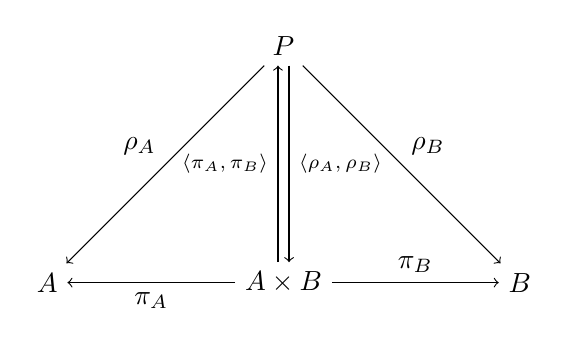
\begin{tikzpicture}[auto]
				\node (a) at (0, 0) {$A$};
				\node (ab) at (3, 0) {$A\times B$};
				\node (b) at (6, 0) {$B$};
				\node (p) at (3, 3) {$P$};
				\draw[->] (p) to node[swap]{$\rho_A$}(a);
				\draw[->] (p) to node{$\rho_B$}(b);
				\draw[->,transform canvas={xshift=2pt}] (p) to node{\scriptsize{$\tuple{\rho_A,\rho_B}$}}(ab);
				\draw[->,transform canvas={xshift=-2pt}] (ab) to node{\scriptsize{$\tuple{\pi_A,\pi_B}$}}(p);
				\draw[->] (ab) to node{$\pi_A$}(a);
				\draw[->] (ab) to node{$\pi_B$}(b);
			\end{tikzpicture}
		\end{center}
		ここで、射$\mor{\tuple{\rho_A,\rho_B}\circ\tuple{\pi_A,\pi_B}}{A\times B}{A\times B}$を射の対とする積の図式を考える、つまり積$(A\times B,\pi_A,\pi_B)$において対$(X,f,g)$に$(A\times B,\pi_A,\pi_B)$を当てはめると二つの射の対の可換性からこの積図式も可換になり、射$\tuple{\rho_A,\rho_B}\circ\tuple{\pi_A,\pi_B}$は実際に射の対になる。ここで恒等射$\mor{id_{A\times B}}{A\times B}{A\times B}$は同様に図式を可換にするから$id_{A\times B}$もまた射の対になる。

		\begin{center}
			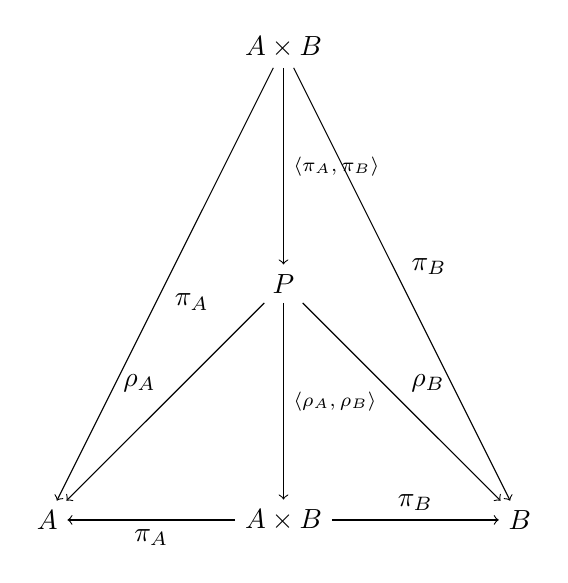
\begin{tikzpicture}[auto]
				\node (a) at (0, 0) {$A$};
				\node (ab) at (3, 0) {$A\times B$};
				\node (ab2) at (3, 6) {$A\times B$};
				\node (b) at (6, 0) {$B$};
				\node (p) at (3, 3) {$P$};
				\draw[->] (p) to node[swap]{$\rho_A$}(a);
				\draw[->] (p) to node{$\rho_B$}(b);
				\draw[->] (p) to node{\scriptsize{$\tuple{\rho_A,\rho_B}$}}(ab);
				\draw[->] (ab2) to node{\scriptsize{$\tuple{\pi_A,\pi_B}$}}(p);
				\draw[->] (ab) to node{$\pi_A$}(a);
				\draw[->] (ab) to node{$\pi_B$}(b);
				\draw[->] (ab2) to node{$\pi_A$}(a);
				\draw[->] (ab2) to node{$\pi_B$}(b);
			\end{tikzpicture}
			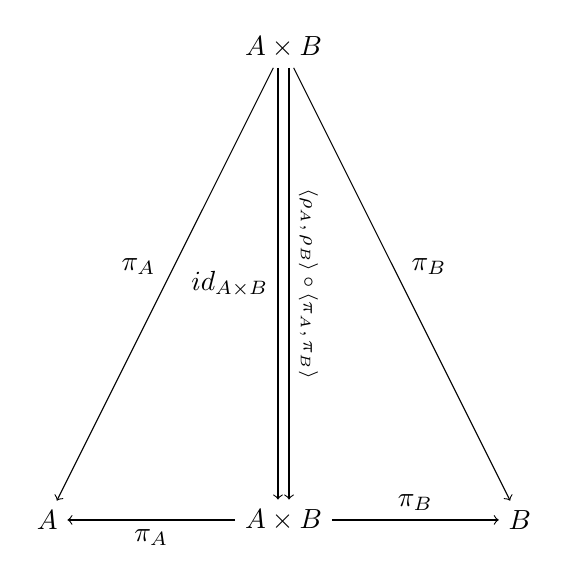
\begin{tikzpicture}[auto]
				\node (a) at (0, 0) {$A$};
				\node (ab) at (3, 0) {$A\times B$};
				\node (b) at (6, 0) {$B$};
				\node (ab2) at (3, 6) {$A\times B$};
				\draw[->] (ab2) to node[swap]{$\pi_A$}(a);
				\draw[->] (ab2) to node{$\pi_B$}(b);
				\draw[->,transform canvas={xshift=2pt}] (ab2) to node[sloped]{\scriptsize{$\tuple{\rho_A,\rho_B}\circ\tuple{\pi_A,\pi_B}$}}(ab);
				\draw[->,transform canvas={xshift=-2pt}] (ab2) to node[swap]{$id_{A\times B}$}(ab);
				\draw[->] (ab) to node{$\pi_A$}(a);
				\draw[->] (ab) to node{$\pi_B$}(b);
			\end{tikzpicture}
		\end{center}

			$\pi_A$、$\pi_B$に対する射の対は一意に定まるから$\tuple{\rho_A,\rho_B}\circ\tuple{\pi_A,\pi_B}=id_{A\times B}$が成り立つ。

			同様に射$\mor{\tuple{\pi_A,\pi_B}\circ\tuple{\rho_A,\rho_B}}{P}{P}$を射の対とする積の図式を考えると、$\tuple{\pi_A,\pi_B}\circ\tuple{\rho_A,\rho_B}=id_{P}$が成り立つ。
			すると$\tuple{\pi_A,\pi_B}$と$\tuple{\rho_A,\rho_B}$はそれぞれ同型射になり、同型射の存在が示せたので$A\times B\cong P$を示せた。
	\end{proof}
		積の一意性の証明では、ある積に対して別の積の射影射の対を取ったが、自身の射影射の対を取るとどうなるのか考えてみ。
	\begin{prop}[射影射の対]
		ある積$(A\times B,\pi_A,\pi_B)$に対して$\tuple{\pi_A,\pi_B}=id_{A\times B}$が成り立つ。
	\end{prop}
	\begin{proof}
		積$(A\times B,\pi_A,\pi_B)$に対して組$(X,f,g)$に$(A\times B,\pi_A,\pi_B)$を当てはめる。
		すると、$\pi_{A}\circ id_{A\times B}=\pi_{A}$と$\pi_{B}\circ id_{A\times B}=\pi_{B}$が成り立つから、$id_{A\times B}$は$\pi_A$と$\pi_B$の対になる。よって射の対の一意性より、$\tuple{\pi_A,\pi_B}=id_{A\times B}$が成り立つ。
		\begin{center}
			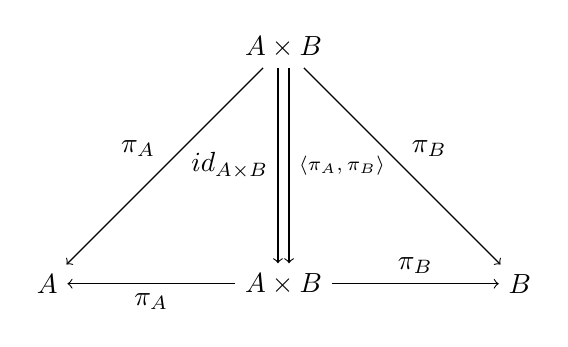
\begin{tikzpicture}[auto]
				\node (a) at (0, 0) {$A$};
				\node (ab) at (3, 0) {$A\times B$};
				\node (b) at (6, 0) {$B$};
				\node (p) at (3, 3) {$A\times B$};
				\draw[->] (p) to node[swap]{$\pi_A$}(a);
				\draw[->] (p) to node{$\pi_B$}(b);
				\draw[->,transform canvas={xshift=2pt}] (p) to node{\scriptsize{$\tuple{\pi_A,\pi_B}$}}(ab);
				\draw[->,transform canvas={xshift=-2pt}] (p) to node[swap]{$id_{A\times B}$}(ab);
				\draw[->] (ab) to node{$\pi_A$}(a);
				\draw[->] (ab) to node{$\pi_B$}(b);
			\end{tikzpicture}
		\end{center}
	\end{proof}
	\subsection{終対象}
	\begin{define}[終対象]
		ある圏$\cat{C}$に終対象が存在するとは、ある対象$1$が存在して圏$\cat{C}$の任意の対象$X$に対し射$\mor{!_X}{X}{1}$が一意に存在するときである。

		元とは射の向きが逆であることに注意してほしい。
	\end{define}
	射の対$\mor{\tuple{f,g}}{X}{A\times B}$は射$f,g$に対して一意に存在するのであったが、終対象への射$\mor{!_X}{X}{1}$は対応する射が存在しない。そのため、終対象への射は無条件で一意に存在することになる。
	\begin{prop}[終対象から終対象への射]
		終対象から終対象への射は恒等射ただ一つである。
	\end{prop}
	\begin{proof}
		終対象$1$に対して、終対象から終対象への射$\mor{!_1}{1}{1}$は無条件で一意に定まる。
		すべての対象に恒等射は存在するから、$id_1=!_1$となり、一意に定まる。
		\begin{center}
			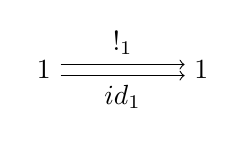
\begin{tikzpicture}[auto]
				\node (1) at (0, 0) {$1$};
				\node (1') at (2, 0) {$1$};
				\draw[->,transform canvas={yshift=2pt}] (1) to node{$!_{1}$}(1');
				\draw[->,transform canvas={yshift=-2pt}] (1) to node[swap]{$id_1$}(1');
			\end{tikzpicture}
		\end{center}
	\end{proof}
	終対象から終対象の射を終対象の元とみなすと、終対象は元がただ一つしかない対象であると分かる。

	\begin{prop}[終対象の一意性]
		終対象$1$に対して別の終対象$1'$が存在するとき、$1\cong 1'$が成り立つ。
	\end{prop}
	\begin{proof}
		終対象$1$における$1'$からの一意に定まる射$\mor{!_1}{1'}{1}$と終対象$1'$における$1$からの一意に定まる射$\mor{{!_1}'}{1}{1'}$の合成$\mor{!_1\circ {!_1}'}{1}{1}$と$\mor{{!_1}'\circ!_1}{1'}{1'}$はそれぞれ終対象から終対象への射である。

		よって$!_1\circ {!_1}'=id_1$と${!_1}'\circ!_1=id_1'$が成り立ち、$!_1$、${!_1}'$が同型射になるから$1\cong 1'$が成り立つ。
		\begin{center}
			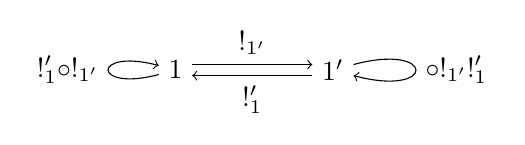
\begin{tikzpicture}[auto]
				\node (1) at (0, 0) {$1$};
				\node (1') at (2, 0) {$1'$};
				\draw[->,transform canvas={yshift=2pt}] (1) to node{$!_{1'}$}(1');
				\draw[->,transform canvas={yshift=-2pt}] (1') to node{$!'_1$}(1);
				\draw[->,loop left ,looseness=20] (1) to node{$!'_1\circ !_{1'}$}(1);
				\draw[->,loop right ,looseness=20] (1') to node{$\circ !_{1'}!'_1$}(1');
			\end{tikzpicture}
		\end{center}
	\end{proof}

	\subsection{演習問題}
	\begin{enumerate}
		\item 対象$A,B$と終対象$1$において、任意の射$\mor{f}{A}{B}$に対して$!_B\circ f=!_A$が成り立つことを示せ。
		\item $A\times 1\cong A$を示せ。(Hint: $\pi_A$と$\tuple{id_A,!_X}$が同型射であることを示せばよい)
	\end{enumerate}
	\section{関手}
	これまでの議論はすべて一つの圏の上で行われてきたが、これからはある圏とまた別の圏の関係について考えていく。
	\begin{define}
		ある圏$\cat{C}$からある圏$\cat{D}$への関手$\functor{F}{C}{D}$は以下の関数と公理から構成される。
		また例として、以下の射と対象で構成される圏$\cat{C},\cat{D}$と二つの関手$\functor{T}{C}{D}$、$\functor{S}{C}{D}$を見ていく。
		\begin{center}
			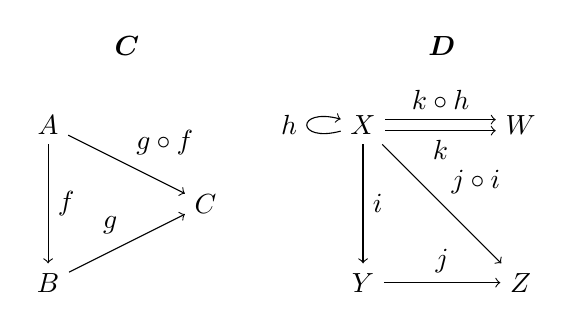
\begin{tikzpicture}[auto]
				\node (a) at (0, 2) {$A$};
				\node (b) at (0, 0) {$B$};
				\node (c) at (2, 1) {$C$};
				\draw[->] (a) to node{$f$}(b);
				\draw[->] (b) to node{$g$}(c);
				\draw[->] (a) to node{$g\circ f$}(c);

				\node (x) at (4, 2) {$X$};
				\node (y) at (4, 0) {$Y$};
				\node (w) at (6, 2) {$W$};
				\node (z) at (6, 0) {$Z$};
				\draw[->] (x) to node{$i$}(y);
				\draw[->] (y) to node{$j$}(z);
				\draw[->] (x) to node{$j\circ i$}(z);
				\draw[->,transform canvas={yshift=-2pt}] (x) to node[swap]{$k$}(w);
				\draw[->,transform canvas={yshift=2pt}] (x) to node{$k\circ h$}(w);
				\draw[->,loop left ,looseness=10] (x) to node{$h$}(x);

				\node (catc) at (1, 3) {$\cat{C}$};
				\node (catd) at (5, 3) {$\cat{D}$};
				%\draw[->,bend right = 15] (catc) to node{$T$}(catd);
				%\draw[->,bend left = 15] (catc) to node{$S$}(catd);
			\end{tikzpicture}
		\end{center}
		\begin{description}
		\item[対象関数]$\cat{C}$の対象$A$に$\cat{D}$の対象$FA$を割り当てる対象関数$\mor{F}{Obj(\cat{C})}{Obj(\cat{D})}$。
		関手$T$の対象関数$T$を\[T(A)=X,\ T(B)=Y,\ T(C)=Z\]と定義する。
		また関手$S$の対象関数$S$を\[S(A)=X,\ S(B)=X,\ S(C)=W\]と定義する。
		\item[射関数]$\cat{C}$の任意の射$\mor{f}{A}{B}$に圏$\cat{D}$の射$\mor{Ff}{FA}{FB}$を割り当てる射関数$\mor{F}{Mor(A,B)}{Mor(FA,FB)}$。対象関数と射関数は記法で区別しないことと、$Tf$ののようにかっこを省略する場合もあることに注意してほしい。

		関手$T$の射関数$T$を\[T(f)=i,\ T(g)=j,\ T(g\circ f)=j\circ i\]と定義する。また各対象の恒等射の対応は
		\begin{align*}
			T(id_A)&=id_{TA}\\
			&=id_{X} \text{($TA=X$)}\\
			T(id_B)&=id_{TB}\\
			&=id_{Y} \text{($TB=Y$)}\\
			T(id_C)&=id_{TC}\\
			&=id_{Z} \text{($TC=Z$)}
		\end{align*}とする。
		\begin{center}
			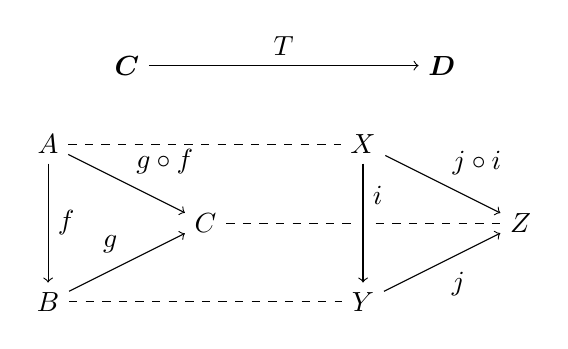
\begin{tikzpicture}[auto]
				\node (a) at (0, 2) {$A$};
				\node (b) at (0, 0) {$B$};
				\node (c) at (2, 1) {$C$};
				\node (x) at (4, 2) {$X$};
				\node (y) at (4, 0) {$Y$};
				\node (z) at (6, 1) {$Z$};
				\draw[-,dashed] (a) to (x);
				\draw[-,dashed] (b) to (y);
				\draw[-,dashed] (c) to (z);

				\draw[->] (a) to node{$f$}(b);
				\draw[->] (b) to node{$g$}(c);
				\draw[->] (a) to node{$g\circ f$}(c);

				\draw[-, line width=4pt,draw=white] (x) to (y);
				\draw[->] (x) to node[yshift =10]{$i$}(y);
				\draw[->] (y) to node[swap]{$j$}(z);
				\draw[->] (x) to node{$j\circ i$}(z);
				\node (catc) at (1, 3) {$\cat{C}$};
				\node (catd) at (5, 3) {$\cat{D}$};
				\draw[->] (catc) to node{$T$}(catd);

			\end{tikzpicture}
		\end{center}
		この図での点線は対象の写像的な対応を表しているのであって、実際に射が存在するわけではないことに注意してほしい。
		関手$S$の射関数$S$を\[S(f)=h,\ S(g)=k,\ S(g\circ f)=k\circ h\]と定義する。
		恒等射の対応は
		\begin{align*}
			S(id_A)&=id_{SA}\\
			&=id_{X} \text{($SA=X$)}\\
			S(id_B)&=id_{SB}\\
			&=id_{X} \text{($SB=X$)}\\
			S(id_C)&=id_{SC}\\
			&=id_{W} \text{($SC=W$)}
		\end{align*}
		とする。
		\begin{center}
			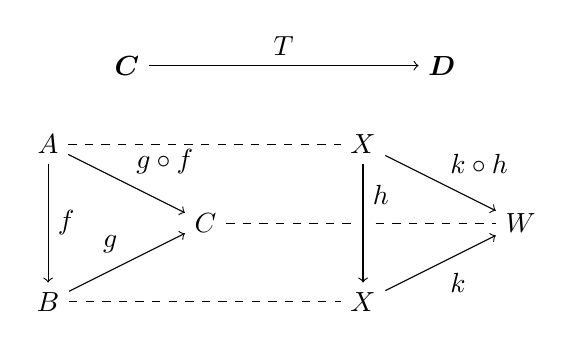
\begin{tikzpicture}[auto]
				\node (a) at (0, 2) {$A$};
				\node (b) at (0, 0) {$B$};
				\node (c) at (2, 1) {$C$};
				\node (x) at (4, 2) {$X$};
				\node (y) at (4, 0) {$X$};
				\node (z) at (6, 1) {$W$};
				\draw[-,dashed] (a) to (x);
				\draw[-,dashed] (b) to (y);
				\draw[-,dashed] (c) to (z);

				\draw[->] (a) to node{$f$}(b);
				\draw[->] (b) to node{$g$}(c);
				\draw[->] (a) to node{$g\circ f$}(c);

				\draw[-, line width=4pt,draw=white] (x) to (y);
				\draw[->] (x) to node[yshift =10]{$h$}(y);
				\draw[->] (y) to node[swap]{$k$}(z);
				\draw[->] (x) to node{$k\circ h$}(z);
				\node (catc) at (1, 3) {$\cat{C}$};
				\node (catd) at (5, 3) {$\cat{D}$};
				\draw[->] (catc) to node{$T$}(catd);

			\end{tikzpicture}
		\end{center}
		\item[恒等射の保存] 射関数は圏$\cat{C}$の恒等射を$\cat{D}$の恒等射に対応させる。つまり$F(id_A)=id_{FA}$が成り立つ。

		関手$T,S$でも定義を見れば成り立つことがすぐに分かる。
		\item[射の合成の保存]$cod(f)=dom(g)$であるとき、$F(g\circ f)=Fg\circ Ff$が成り立つ。

		関手$T,S$においてそれぞれ
		\begin{align*}
			T(g\circ f)&=j\circ i&\text{($T(g\circ f)$の定義)}\\
			&=Tg\circ Tf&\text{($Tg,Tf$の定義)}\\
			S(g\circ f)&=k\circ h&\text{($S(g\circ f)$の定義)}\\
			&=Sg\circ Sf&\text{($Sg,Sf$の定義)}
		\end{align*}
		が成り立つから射の合成を保つことがわかる。
		\end{description}
	\end{define}
	\begin{prop}[図式の圏論的な定義]
		添字圏と呼ばれる圏$\cat{J}$から図式を取りたい圏$\cat{C}$への関手は図式である。
		例えば以下のように対象$I,J,K$と射$i,j$で構成される添字圏$J$を図式の骨組み、関手$\functor{F}{I}{C}$を図式の骨組みに圏$C$の対象と射を割り当てる操作とする。

		実際に図式に求められる性質は関手の定義によって満たされることがわかる。
		\begin{center}
			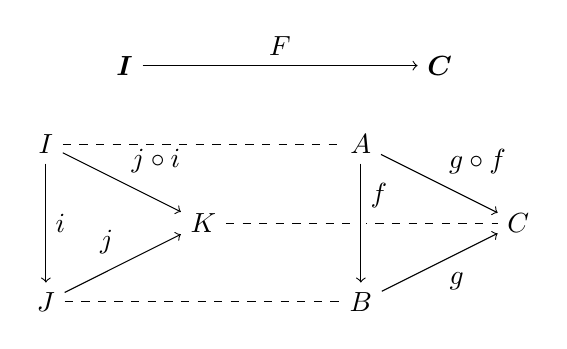
\begin{tikzpicture}[auto]
				\node (a) at (0, 2) {$I$};
				\node (b) at (0, 0) {$J$};
				\node (c) at (2, 1) {$K$};
				\node (x) at (4, 2) {$A$};
				\node (y) at (4, 0) {$B$};
				\node (z) at (6, 1) {$C$};
				\draw[-,dashed] (a) to (x);
				\draw[-,dashed] (b) to (y);
				\draw[-,dashed] (c) to (z);

				\draw[->] (a) to node{$i$}(b);
				\draw[->] (b) to node{$j$}(c);
				\draw[->] (a) to node{$j\circ i$}(c);

				\draw[-, line width=4pt,draw=white] (x) to (y);
				\draw[->] (x) to node[yshift =10]{$f$}(y);
				\draw[->] (y) to node[swap]{$g$}(z);
				\draw[->] (x) to node{$g\circ f$}(z);
				\node (catc) at (1, 3) {$\cat{I}$};
				\node (catd) at (5, 3) {$\cat{C}$};
				\draw[->] (catc) to node{$F$}(catd);

			\end{tikzpicture}
		\end{center}
	\end{prop}
	\begin{define}[積関手]
		以下の関数で構成されるある対象$B$に対して圏$C$から圏$C$への関手$\functor{-\times B}{C}{C}$を積関手と呼ぶ。
		\begin{description}
			\item[対象関数] 対象関数を$(-\times B)(A)=A\times B$と定義する。
			\item[射関数] 圏$C$の任意の対象$A,A'$と任意の射$\mor{f}{A}{A'}$に対して射関数を\[\mor{(-\times B)(f)=f\times id_B}{A\times B}{A'\times B}\]と定義する。
			\begin{center}
				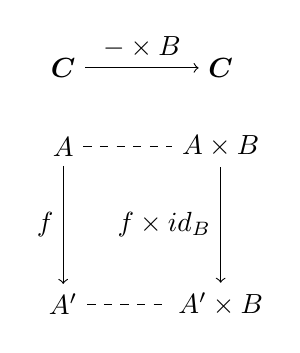
\begin{tikzpicture}[auto]
					\node (a) at (0, 2) {$A$};
					\node (a') at (0, 0) {$A'$};
					\node (ab) at (2, 2) {$A\times B$};
					\node (a'b) at (2, 0) {$A'\times B$};
					\node (catc1) at (0, 3) {$\cat{C}$};
					\node (catc2) at (2, 3) {$\cat{C}$};
					\draw[-,dashed] (a) to (ab);
					\draw[-,dashed] (a') to (a'b);

					\draw[->] (catc1) to node{$-\times B$}(catc2);
					\draw[->] (a) to node[swap]{$f$}(a');
					\draw[->] (ab) to node[swap]{$f\times id_B$}(a'b);
				\end{tikzpicture}
			\end{center}
			\item[恒等射の保存] $(-\times B)(id_A)=id_{(-\times B)(A)}$を示せばよい。
			\begin{align*}
				(-\times B)(id_A)&=id_A\times id_B&\text{(射関数の定義)}\\
				&=\tuple{id_A\circ\pi_A,id_B\circ\pi_B}&\text{(射の積の定義)}\\
				&=\tuple{\pi_A,\pi_B}&\text{(恒等射の性質)}\\
				&=id_{A\times B}&\text{(射影射の対)}\\
				&=id_{(-\times B)(A)}&\text{(対象関数の定義)}
			\end{align*}
			よって積関手は恒等射を保つことが示せた。
			\item[射の合成の保存]任意の対象$A,A',A''$と任意の射$\mor{f}{A}{A'},\mor{f'}{A'}{A''}$に対して\[(-\times B)(f'\circ f)=(-\times B)(f')\circ(-\times B)(f)\]が成り立つことを示せばよい。
			\begin{align*}
				(-\times B)(f'\circ f)&=(f'\circ f)\times id_B&\text{(射関数の定義)}\\
				&=(f'\circ f)\times (id_B\circ id_B)&\text{(恒等射の性質)}\\
				&=(f'\times id_B)\circ(f\times id_B)&\text{(積と合成の交換)}\\
				&=(-\times B)(f')\circ(-\times B)(f)&\text{(射関数の定義)}
			\end{align*}
			\begin{center}
				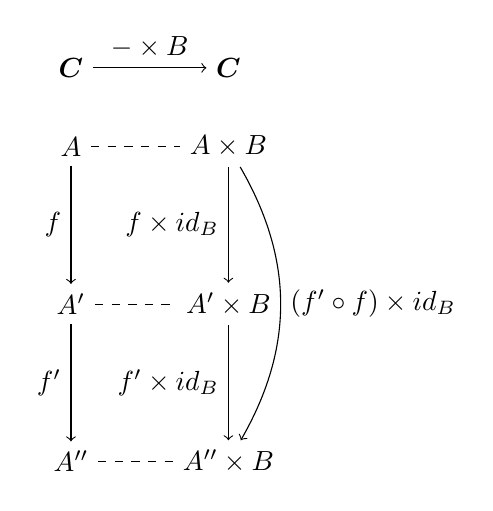
\begin{tikzpicture}[auto]
					\node (a) at (0, 2) {$A$};
					\node (a') at (0, 0) {$A'$};
					\node (a'') at (0, -2) {$A''$};
					\node (ab) at (2, 2) {$A\times B$};
					\node (a'b) at (2, 0) {$A'\times B$};
					\node (a''b) at (2, -2) {$A''\times B$};
					\node (catc1) at (0, 3) {$\cat{C}$};
					\node (catc2) at (2, 3) {$\cat{C}$};
					\draw[-,dashed] (a) to (ab);
					\draw[-,dashed] (a') to (a'b);
					\draw[-,dashed] (a'') to (a''b);
					\draw[->] (catc1) to node{$-\times B$}(catc2);
					\draw[->] (a) to node[swap]{$f$}(a');
					\draw[->] (a') to node[swap]{$f'$}(a'');
					\draw[->] (ab) to node[swap]{$f\times id_B$}(a'b);
					\draw[->] (a'b) to node[swap]{$f'\times id_B$}(a''b);
					\draw[->,bend left =30] (ab) to node{$(f'\circ f)\times id_B$}(a''b);
				\end{tikzpicture}
			\end{center}
			よって積関手は射の合成を保つことが示せた。
		\end{description}
	\end{define}
	関手は二つの関数から構成されるから、これらの関数の合成によって関手の合成が定義できそうである。
	さてこの合成関手が実際に関手になるか確かめる。
	\begin{define}[合成関手]
		関手$\functor{F}{C}{C'}$、$\functor{G}{C'}{C''}$を合成した関手$\functor{G\circ F}{C}{C'}$を以下の要素によって定義する。
		\begin{description}
			\item[対象関数]関手$F,G$のそれぞれの対象関数$F,G$に対して$G\circ F$の対象関数を$G\circ F$と定義する。
			つまり圏$\cat{C}$の任意の対象$A$に対して$(G\circ F)(A)=G(FA)$となるような関数である。
			\item[射関数]関手$F,G$のそれぞれの射関数$F,G$に対して$G\circ F$の射関数もまた$G\circ F$と定義する。
			つまり圏$\cat{C}$の任意の対象$A,A'$と任意の射$\mor{f}{A}{A'}$に対して\[\mor{(G\circ F)(f)=G(Ff)}{GFA}{GF{A'}}\]となるような関数である。
			\begin{center}
				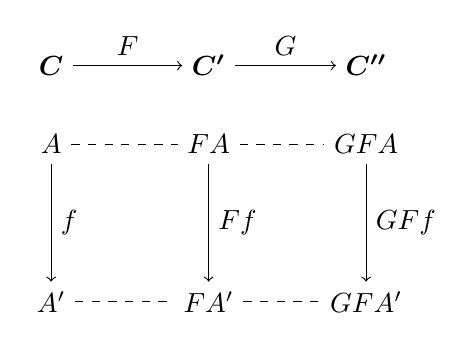
\begin{tikzpicture}[auto]
					\node (a) at (0, 2) {$A$};
					\node (a') at (0, 0) {$A'$};
					\node (fa) at (2, 2) {$FA$};
					\node (fa') at (2, 0) {$FA'$};
					\node (gfa) at (4, 2) {$GFA$};
					\node (gfa') at (4, 0) {$GFA'$};
					\node (catc) at (0, 3) {$\cat{C}$};
					\node (catc') at (2, 3) {$\cat{C'}$};
					\node (catc'') at (4, 3) {$\cat{C''}$};
					\draw[-,dashed] (a) to (fa);
					\draw[-,dashed] (a') to (fa');
					\draw[-,dashed] (fa) to (gfa);
					\draw[-,dashed] (fa') to (gfa');
					\draw[->] (catc) to node{$F$}(catc');
					\draw[->] (catc') to node{$G$}(catc'');

					\draw[->] (a) to node{$f$}(a');
					\draw[->] (fa) to node{$Ff$}(fa');
					\draw[->] (gfa) to node{$GFf$}(gfa');

				\end{tikzpicture}
			\end{center}
			また紛らわしくない場合は合成関手$G\circ F$を$GF$と略すことにする。
			\item[恒等射の保存] $GF(id_A)=id_{GFA}$を示せばよい。
				\begin{align*}
					GF(id_A)&=G(F(id_A))&\text{(射関数の定義)}\\
					&=G(id_{FA})&\text{(関手$F$の恒等射の保存)}\\
					&=id_{GFA}&\text{(関手$G$の恒等射の保存)}
				\end{align*}
			よって合成関手は恒等射を保つ。
			\item[射の合成の保存] $GF(g\circ f)=GFg\circ GFf$を示せばよい。
				\begin{align*}
					GF(g\circ f)&=G(F(g\circ f))&\text{(射関数の定義)}\\
					&=G(Fg\circ Ff)&\text{(関手$F$の射の合成の保存)}\\
					&=GFg\circ GFf&\text{(関手$G$の射の合成の保存)}
				\end{align*}
			よって合成関手は射の合成を保つ。
			\begin{center}
				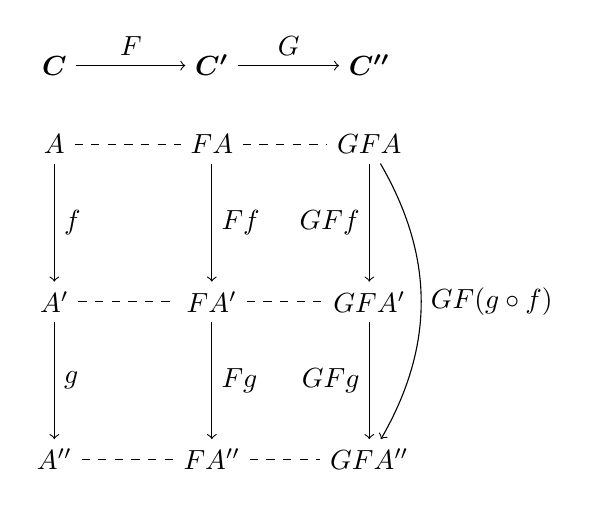
\begin{tikzpicture}[auto]
					\node (a) at (0, 2) {$A$};
					\node (a') at (0, 0) {$A'$};
					\node (a'') at (0, -2) {$A''$};
					\node (fa) at (2, 2) {$FA$};
					\node (fa') at (2, 0) {$FA'$};
					\node (fa'') at (2, -2) {$FA''$};
					\node (gfa) at (4, 2) {$GFA$};
					\node (gfa') at (4, 0) {$GFA'$};
					\node (gfa'') at (4, -2) {$GFA''$};
					\node (catc) at (0, 3) {$\cat{C}$};
					\node (catc') at (2, 3) {$\cat{C'}$};
					\node (catc'') at (4, 3) {$\cat{C''}$};
					\draw[-,dashed] (a) to (fa);
					\draw[-,dashed] (a') to (fa');
					\draw[-,dashed] (a'') to (fa'');
					\draw[-,dashed] (fa) to (gfa);
					\draw[-,dashed] (fa') to (gfa');
					\draw[-,dashed] (fa'') to (gfa'');
					\draw[->] (catc) to node{$F$}(catc');
					\draw[->] (catc') to node{$G$}(catc'');

					\draw[->] (a) to node{$f$}(a');
					\draw[->] (a') to node{$g$}(a'');

					\draw[->] (fa) to node{$Ff$}(fa');
					\draw[->] (fa') to node{$Fg$}(fa'');

					\draw[->] (gfa) to node[swap]{$GFf$}(gfa');
					\draw[->] (gfa') to node[swap]{$GFg$}(gfa'');
					\draw[->,bend left =30] (gfa) to node{$GF(g\circ f)$}(gfa'');
				\end{tikzpicture}
			\end{center}
		\end{description}
	\end{define}
	\subsection{小さい圏の圏}
	\begin{define}[小さい圏の圏]
		小さい圏の圏$\catcat$は以下の要素で構成される
		\begin{description}
			\item[対象] 任意の小さい圏
			\item[射] 任意の圏$\cat{A,B}$の間の任意の関手$\functor{F}{A}{B}$
			\item[射の合成] 関手$\functor{F}{C}{C'}$、$\functor{G}{C'}{C''}$を合成した関手$\functor{G\circ F}{C}{C'}$を定義する。
			対象関数と射関数をそれぞれ$(G\circ F)(X)=G(FX)$、$(G\circ F)(f)=G(Ff)$のように
			$F\circ G$の対象関数、射関数をそれそれ
			\item[恒等射の存在]
			\item[結合律]
			\item[単位元律]
		\end{description}
	\end{define}
	\begin{define}[一点離散圏]
		content...
	\end{define}
	\begin{prop}[$\catcat$の終対象]
		$\cat{1}$は$\catcat$における終対象である。
	\end{prop}
	\begin{define}[積圏]

	\end{define}
	\subsection{反変関手}
	\subsection{表現可能関手}
	\section{自然変換}
	\section{随伴関手}
	\section{デカルト閉圏}
	\section{米田の補題}

	\begin{thebibliography}{99}
	\bibitem{1} S.マックレーン, (2019)『圏論の基礎』(三好博之・高木理訳)丸善出版
	\bibitem{2} Steve Awodey, (2016)『圏論-原書第2版』(前原和寿訳)共立出版
	\bibitem{3} 壱大整域 \url{http://alg-d.com/math/kan_extension/}
	\bibitem{4} nLab \url{https://ncatlab.org/nlab/show/HomePage}
	\bibitem{5} Category Theory for Programmers: The Preface \url{https://bartoszmilewski.com/2014/10/28/category-theory-for-programmers-the-preface/}
	\end{thebibliography}


\end{document}
